\documentclass[a4paper, 11pt]{article}
    \usepackage{CJKutf8}
    \usepackage{geometry}
    \usepackage[utf8]{inputenc}
    \usepackage[colorlinks, linkcolor=blue]{hyperref}
    \usepackage[linesnumbered, boxed, ruled, commentsnumbered]{algorithm2e}
    \usepackage{graphicx}
    \usepackage{diagbox}
    \graphicspath{ {figures/} }
    \title{区块链安全综述}
    \author{林文海(11721018)}
    \date{2018年06月10日}
    
    \begin{document}
    \setlength\parindent{2em}

        %%%% 重定义 %%%%
        \renewcommand{\contentsname}{目录}  % 将Contents改为目录
        \renewcommand{\abstractname}{摘要}  % 将Abstract改为摘要
        \renewcommand{\refname}{参考文献}   % 将References改为参考文献
        \renewcommand{\indexname}{索引}
        \renewcommand{\figurename}{图}
        \renewcommand{\tablename}{表}
        \renewcommand{\appendixname}{附录}
    
    \begin{CJK*}{UTF8}{gbsn}

    \maketitle
    
    \begin{abstract}
        这是中文摘要。这是中文摘要。这是中文摘要。这是中文摘要。这是中文摘要。这是中文摘要。这是中文摘要。
        这是中文摘要。这是中文摘要。这是中文摘要。这是中文摘要。这是中文摘要。这是中文摘要。这是中文摘要。这是中文摘要。
        这是中文摘要。这是中文摘要。这是中文摘要。这是中文摘要。这是中文摘要。这是中文摘要。这是中文摘要。这是中文摘要。
    \end{abstract}

    \renewcommand{\abstractname}{Abstract}

    \begin{abstract}
        This is abstract in English.This is abstract in English.This is abstract in English.
        This is abstract in English.This is abstract in English.This is abstract in English.
        This is abstract in English.This is abstract in English.This is abstract in English.
    \end{abstract}

    \section{前言}

    \indent

    比特币\cite{ref_article1}是第一个完全去中心化的电子货币系统。
    自从比特币在2009发行以来,
    它的价值已经获得巨大的提升,
    截止2018年6月10日,
    单个比特币的价值为
    7311.87美元,
    比特币总市值已经突破1249亿美元\cite{ref_web1}。


    比特币以去中心化以及安全性著称,
    但事实上依然存在着可以被人利用的漏洞,
    本文对近几年来针对比特币挖矿攻击的研究进行了归纳概括,
    其中主要介绍Selfish Mining攻击\cite{ref_selfish_mining1, ref_selfish_mining2, ref_selfish_mining3}、
    BWH攻击\cite{ref_BWH1, ref_BWH2, ref_article3}以及FAW攻击\cite{ref_FAW}。本文的组织结构如下:
    \begin{itemize}
        \item 第一节前沿介绍背景以及本文的综述内容。
        \item 第二节介绍本文需要的比特币基础知识,包括比特币基本原理、挖矿过程以及区块链分叉。
        \item 第三、四、五分别介绍了Selfish Mining攻击、BWH攻击和FAW攻击,具体包括攻击的基本原理、攻击效果、攻击的改进版本、如何预防攻击等。
        \item 第六节对全文进行总结。

    \end{itemize}

    \section{比特币基础}

    \indent
    
    比特币的核心是基于区块链技术,
    区块链本质上是一种分布式账本,
    它记录着比特币系统的所有历史交易信息。
    为了保证分布式账本的内容不会被随意篡改,
    比特币系统需要网络中的P2P节点使用它们的算力
    去解决某种哈希计算题,
    以此来产生工作量证明PoW,
    想要产生一个区块同时将交易加入到区块中就必须要有PoW。
    我们将产生区块的过程称为“挖矿”,
    参与挖矿的P2P节点我们称之为“矿工”。
    当矿工挖出一个新的区块后会立即把新区块通过比特币网络进行广播并开始下一轮的挖矿,
    其他节点会对新区块进行校验,如果校验合法,那么新区块
    将被加入到原有的区块链的头,
    从而延长整个区块链。
    如果矿工挖出来的块获得网络上大多数节点的认可,
    那么矿工将获得一些比特币作为奖励。
    新的区块中的头保存着前一个区块的哈希值,
    如果前一个区块内容发生改变,
    那么将要重新进行PoW,
    并且导致后面的区块内容也发生变化,
    也要重新进行PoW。
    因此,随着区块链越来越长,
    篡改越早以前的区块的代价将越大,
    这就保证了区块链上数据具有不可篡改的特性。


    截止2018年06月,
    每挖到一个新区块的矿工将获得最少12.5个比特币作为奖励,
    除此之外,新区块中包含的所有
    交易的手续费也将作为矿工的奖励。
    根据比特币的设计,
    新区块的产生速度需要保持在平均每10分钟一个,
    由于比特币网络的总的计算
    能力在不停的变化,
    因此挖矿的难度需要频繁进行调整,
    这个周期为两周,
    准确地说是产生2016个区块花费的时间。
    随着挖矿难度的提升,
    独立矿工挖到新区块的平均时间将变得更长,
    并且很不稳定。
    为了避免这种收入不稳定的问题,
    一些矿工就组织共同进行挖矿并根据算力分享收益,这被称为矿池。
    大部分矿池由矿池管理着和矿工构成。
    管理者作为比特币网络上的节点运行完整的比特币协议,
    而矿工是通过运行矿池协议\cite{ref_web2}
    加入矿池而不是直接连接到比特币网络上。
    矿池管理者将未解决的挖矿任务分成一个个子任务分给矿工,
    矿工解决这些子任务后将产生PPoW和FPoW,
    并将他们提交给矿池管理者。
    PPoW是指没有挖出新的区块但是验证了一部分答案是错误的,
    FPoW是指找到了正确答案,也就是挖到区块。
    如果一个矿池中的矿工产生了FPoW并将它提交给管理者,
    管理者会立即将FPoW产生的新区块广播到比特币网络中。
    如果区块经过了其他大部分节点的验证并被采纳,
    那么矿池管理者将受到奖励,
    同时按照矿工贡献的PoW的比例将奖励分给矿工。
    比特币网络(挖矿部分)当前由独立矿工、允许任何人加入的开放矿池以及需要认证才能加入的私人矿池构成。

    
    \subsection{比特币挖矿过程}

    \indent

    区块链中的交易是以Merkle树\cite{ref_article2}的结构存储在区块中。
    区块链中每一个区块的头都包含了当前区块Merkle树根的哈希值、前一个区块的头哈希值、难度目标以及nonce值。
    在比特币系统中,挖矿其实就是不断地尝试nonce值,
    然后计算加密问题以此产生PoW。
    具体来说,挖矿的目标就是找到一个有效的nonce值满足$\ sha256(sha256(blkhdr)) < t $,
    其中 $\ blkhdr$ 是区块完整的头信息,
    $\ t$是一个根据比特币协议计算出来的256位的数值,称为难度目标。
    因为哈希计算是不可逆的,因此矿工只能通过不断的尝试nonce值来计算区块头的哈希,
    很明显这个的难度是很高的。
    为了保证区块的平均产生速度在10分钟左右,
    比特币系统每产生2016个区块后都要重新调整难度目标 $\ t$ 的值。
    当一个矿工发现一个有效的nonce值并且产生一个新的区块后会立即将新区块广播给比特币网络中的每个节点。
    当其他节点接收到新区块并通过验证后,
    会把新区块作为区块链的新的头。

    \subsection{区块链分叉}

    \indent

    比特币系统中的区块链分叉分为由挖矿产生的分叉\cite{ref_web3}和由版本升级产生的分叉\cite{ref_web4},
    而由版本升级产生的分叉又分为软分叉和硬分叉,
    我们这里提到的分叉特指由挖矿产生的分叉,
    当两个矿工在很短的时间内相继挖到了有效的新的区块并将新区块广播到比特币网络上,
    由于网络存在延时,
    因此有些节点先收到了区块 $\ B_1$,
    而有些节点先收到了区块 $\ B_2$,
    通常情况下,
    节点会将先收到的区块作为区块链的新的头。
    所以,整个网络中就存在着一部分节点以区块$\ B_1$作为区块链的头而
    其他节点以区块$\ B_2$作为区块链的头,这就是由挖矿所产生的区块链分叉。
    在产生分叉后的新一轮挖矿中,
    会有一个分叉先算出来新的区块,
    那么这个分叉就是有效的,
    而另一个分叉是无效的。
    除了这种偶然产生的分叉外,
    分叉也可以人为地故意产生。
    当一个矿工先挖出了一个新区块但是不立即将其广播到网络上,
    知道矿工检测到网络中其他的节点也挖出了一个新的区块后才将自己的挖到的新区块广播出去,
    以此来故意产生分叉。
    这种故意产生的分叉可以被用于“双重支付”攻击\cite{ref_double_spending}和“selfish mining”攻击
    \cite{ref_selfish_mining1, ref_selfish_mining2, ref_selfish_mining3}。

    \section{Selfish Mining}

    \indent

    正常情况下,一个诚实的矿工产生一个FPoW后会立即将新区块广播到比特币网络上,
    但是在selfish mining攻击\cite{ref_selfish_mining1}中,
    攻击者不会立即将新区块广播出去,
    此时攻击者可以偷偷地开始挖新的区块,
    而其他诚实的矿工还在原有的公链上挖矿。
    如果攻击者发现了更多的新区块,
    就继续偷偷地往后面挖新区块。
    当公共分支的长度达到了私有分支的长度时,
    攻击者就将自己发现的新区快全部广播出去。

    \subsection{攻击原理}

    \indent

    Selfish mining攻击的核心思想就是使其他的诚实矿工在已经输掉的挖矿比赛中继续浪费算力。
    具体来说就是攻击者使得诚实的矿工将部分算力花在挖掘不可能成为区块链一部分的区块上,
    因为这一高度的区块早已经被攻击者挖到了。

    Selfish mining攻击者通过选择合适的时机发布自己挖到的区块从而使其他诚实的矿工做了无用的工作。
    通俗来讲,
    攻击者偷偷保存自己挖到的区块,
    然后人为地产生分叉,
    并在自己的这条私有的分叉上继续挖矿,
    然而诚实的矿工却还在较短原有的公共链上挖矿。
    因为攻击者的算力只占全网算力的一小部分,
    因此私有分叉的长度不会一直领先于公有链长度。
    所以,攻击者必须选择合适的时机将新区块发布出去,
    使得诚实的矿工放弃在原有的公链上挖矿而从新的区块开始挖,
    从而达到攻击的目的。
    这使得诚实矿工在公链上挖矿的工作都白费了,
    反过来就增加了攻击者的收入。

    根据这种思路,selfish mining策略的算法如算法 \ref{algorithm:selfishMine}所示。
    这个策略是由攻击者和诚实的矿工的挖矿事件驱动的,
    每一步的决策都取决于攻击者的私有链以及公链的长度。
    接下来将结合具体的场景介绍selfish mining的策略。

    首先是第一种最简单的情况,
    当公链的长度比攻击者的私有链的长度长。
    由于攻击者的算力一定是小于全网其他节点的算力之和,
    所以攻击者私有链的长度赶上并超过公链的概率是非常非常低的,
    因此在这种情况下,攻击者必须让公有链覆盖私有链。

    第二种情况是攻击者先发现了一个新区块,
    导致私有链的长度领先于公有链,
    攻击者占据很大的优势。
    这时候攻击者开始偷偷在新的私有链上挖掘区块而不是马上地把新区块广播出去。
    接下来又会出现两种情况,
    要么诚实的矿工也发现了一个新的区块使得公有链长度与私有链长度一致,
    要么攻击者又先发现了一个区块,使得私有链长度比公有链至少长2。

    \begin{algorithm}
        \caption{Selfish-Mine}
        \label{algorithm:selfishMine}

        \textbf{on} Init

            $\ \ \ \ $ public chain  $\leftarrow$ publickly known blocks

            $\ \ \ \ $ private chain $\leftarrow$ publickly known blocks

            $\ \ \ \ $ \textit{privateBranchLen} $\leftarrow$ 0

            $\ \ \ \ $ Mine at the head of the private chain.

        $ $
        
        \textbf{on} My pool found a block

            $\ \ \ \ $ $\Delta_{\textit{prev}}$ $\leftarrow$ length(private chain) - length(public chain)

            $\ \ \ \ $ append new block to private chain

            $\ \ \ \ $ \textit{privateBranchLen} $\leftarrow$ \textit{privateBranchLen} + 1

            $\ \ \ \ $ \textbf{if} $\Delta_{\textit{prev}} = 0$ \textit{and privateBranchLen} = 2 \textbf{then} \hfill (Was tie with branch of 1)

                $\ \ \ \ \ \ \ \ $ publish all of the private chain \hfill (Pool wins due to the lead of 1)

                $\ \ \ \ \ \ \ \ $ \textit{privateBranchLen} $\leftarrow$ 0
            
            $\ \ \ \ $ Mine at the new head of the private chain.
        
        $ $

        \textbf{on} Others found a block 

            $\ \ \ \ $ $\Delta_{\textit{prev}}$ $\leftarrow$ length(private chain) - length(public chain)
            
            $\ \ \ \ $ append new block to public chain 

            $\ \ \ \ $ \textbf{if} $\Delta_{\textit{prev}} = 0$ \textbf{then}

                $\ \ \ \ \ \ \ \ $ private chain $\leftarrow$ public chain \hfill (they win)

                $\ \ \ \ \ \ \ \ $ \textit{privateBranchLen} $\leftarrow$ 0
            
            $\ \ \ \ $ \textbf{else if} $\Delta_{\textit{prev}} = 1 $ \textbf{then}

                $\ \ \ \ \ \ \ \ $ publish last block of the private chain \hfill (Now same length. Try our luck)

            $\ \ \ \ $ \textbf{else if} $\Delta_{\textit{prev}} = 2 $ \textbf{then}

                $\ \ \ \ \ \ \ \ $ publish all of the private chain \hfill (Pool wins due to the lead of 1)

                $\ \ \ \ \ \ \ \ $ \textit{privateBranchLen} $\leftarrow$ 0
            
            $\ \ \ \ $ \textbf{else} \hfill ($\Delta_{\textit{prev}} > 2$)

                $\ \ \ \ \ \ \ \ $ publish first unpublished block in private block.
            
            $\ \ \ \ $ Mine at the head of the private chain.

    \end{algorithm}

    当诚实的矿工挖到区块时,
    攻击者会立即将自己挖到的新区块广播出去,
    此时便产生了分叉。
    攻击者的所有节点全都会采纳并广播自己挖到的区块,
    而其他的节点则是采纳先接收到的那个区块。
    此时,如果攻击者成功地抢在没有采纳自己挖出区块的矿工之前又挖出了一个区块,
    就立即将区块广播出去并同时获得第一个区块和第二个区块的奖励。
    如果诚实的矿工在采纳了攻击者的区块后挖出了一个新区块,
    那么攻击者能够获得第一个区块而这个矿工获得第二个区块的收益。
    如果诚实的矿工采纳了诚实的矿工挖出的区块后又挖出了第二个区块,
    那么攻击者什么奖励都没有。

    在第二种情况下,攻击者又成功地先挖出了第二个区块,
    此时攻击者的私有链长度比公有链至少长2,
    因此便有了一定的缓冲。
    每当诚实的矿工挖到一个区块,
    攻击者也跟着发布私有链中的第一区块。
    由于攻击者的算力落后于全网其他矿工的算力和,
    因此攻击者的私有链的领先长度最终会缩小为1,
    此时,攻击者再把剩下的区块全部发布出去,
    由于攻击者的链还是比公有链长1,
    因此全网所有节点都会采纳攻击者的区块,
    攻击者便获得了所有区块的奖励然后又开始了新一轮的循环。

    \subsection{仿真结果}

    \indent

    假设selfish mining攻击者的算力为 $ \alpha$ ,
    那么其他诚实的矿工的算力和就是$1 - \alpha$。
    用$\gamma$表示在出现分叉时诚实的矿工选择采纳攻击者的区块的概率,
    反之$1 - \gamma$就表示诚实的矿工选择其他区块的概率。

    Eyal等根据上一节的猜想进行了一系列的理论分析,具体见原文\cite{ref_selfish_mining1}。
    为了验证理论分析的正确,
    原文作者将理论分析的结果与比特币协议仿真器的结果做了对比。
    实验使用了仿真器去模拟1000个矿工以相同的速率挖矿的过程,
    其中$1000\alpha$的矿工构成一个矿池运行Selfish-Mine算法,
    剩下的$1000(1-\alpha)$的矿工作为诚实的矿工运行正常的比特币协议。
    实验假设区块的传播时间相比于挖矿时间可以忽略不计,
    正如现实那样,新区块产生平均需要10分钟,
    而区块的传播时间是百ms级别的。
    当公有链和私有链的长度一样时,
    作者人为地对诚实的矿工进行划分,
    其中 $1000(1-\alpha)\gamma$ 的矿工采纳攻击者的区块,
    剩下的 $1000(1-\alpha)(1-\gamma)$ 的矿工采纳其他区块。
    图\ref{figure:figure1}是理论分析的结果和仿真结果的对比,
    可以看出二者是吻合的。

    \begin{figure}[h]
        \centering
        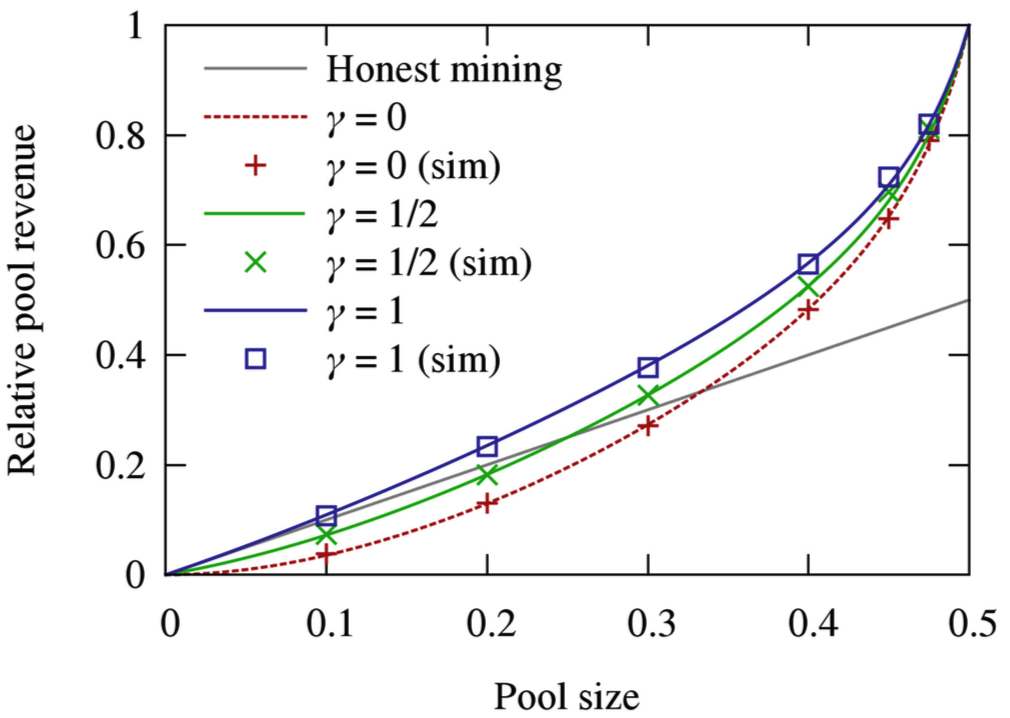
\includegraphics[width=0.6\textwidth]{figure1}
        \label{figure:figure1}
        \caption{在不同的$\gamma$情况下,分别采用正常的挖矿协议和Selfish-Mine算法,攻击者的收益对比。
        从仿真结果和理论分析都可以看出,
        在$\alpha$超过某个阈值时,
        采用Selfish-Mine算法比采用正常的挖矿协议收益要高,
        这个阈值与$\gamma$有关。}
    \end{figure}

    作者根据理论分析发现了两个结论:\\

    \textbf{结论1.} 对于一个确定的$\gamma$,
    当$\alpha$在满足以下范围时采用Selfish-Mine的收益会高于采用正常的挖矿协议。

    \begin{equation}
        \frac{1-\gamma}{3-2\gamma} < \alpha < \frac{1}{2}
    \end{equation}

    可以利用图\ref{figure:figure1}来证明这个结论。
    从图\ref{figure:figure1}可以看出在不同的$\alpha$和$\gamma$的情况下,
    攻击者的收益变化。
    回顾一下前面提到的,
    根据Selfish-Mine算法,
    只有在攻击者只领先公有链一个区块时才需要承担0收益的风险。
    当$\gamma = 1$时,攻击者可以迅速地将自己的区块广播出去并被所有的诚实矿工所采纳,
    那么攻击者便总是能够获得收益而不用承担风险。
    此时只要$\alpha > 0$那么采用Selfish-Mine算法就是有益的。
    当$\gamma = 0$时,诚实的矿工一定不会采纳攻击者的区块,此时必须满足$\alpha > 1/3$。
    当$\gamma = 1/2$时,$\alpha$必须大于1/4。
    图\ref{figure:figure2}表示阈值$\alpha$与$\gamma$的关系。\\

    \textbf{结论2.} 对于一个运行Selfish-Mine算法的矿池来说,
    当矿池的规模大于阈值时,
    矿池中每个成员的收入会随着矿池规模的变大而变大。

    \begin{figure}[h]
        \centering
        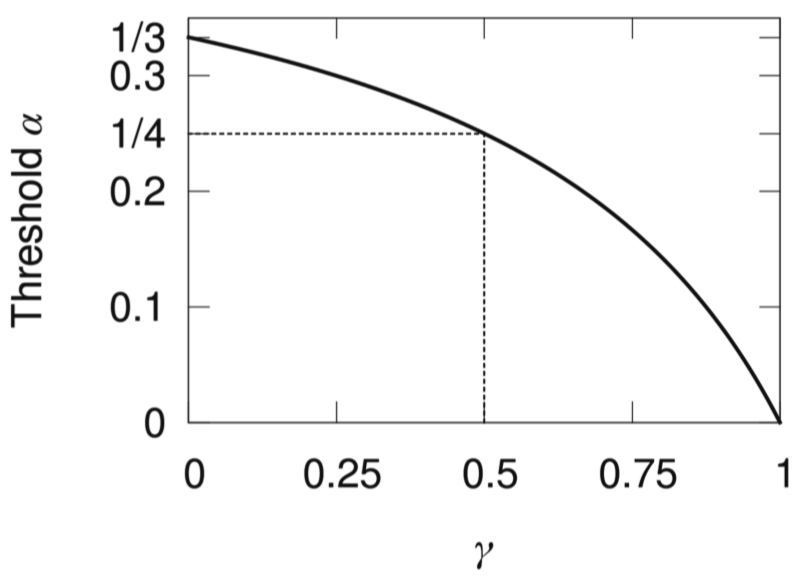
\includegraphics[width=0.6\textwidth]{figure2}
        \caption{对于给定的$\gamma$,$\alpha$是Selfish-Mine算法会胜过正常的挖矿协议的阈值。}
        \label{figure:figure2}
    \end{figure}
    
    \subsection{使用Sybil攻击增强Selfish Mining}

    根据\ref{figure:figure2},
    假设在一个一般的情况下$\gamma = 1/2$,
    此时$\alpha$需要大于1/4才能保证Selfish-Miner获得额外的收益。
    而想要掌握全网1/4算力从而发动攻击其实是一件比较不现实的事情,
    因此降低$\gamma$从而减小$\alpha$成为改善selfish-mining攻击的一个方向。

    Sybil攻击可以实现降低$\gamma$的目标。
    攻击者往比特币网络中加入大量0算力的矿工,
    这些矿工只负责转发区块,
    而不会真正参与挖矿。
    当攻击者的私有链的长度与公有链一样导致产生竞争时,
    这些Sybil矿工只会采纳并转发攻击者产生的区块。
    当Sybil节点数量足够多时,
    $\gamma$会得到显著的下降,
    使得Selfish-Miner只需要很低的算力便可以获得额外的收益。

    \subsection{对抗Selfish Mining}

    由理论分析和仿真结果可以看出,
    阈值$\alpha$和$\gamma$是负相关的,
    但是比特币协议没有任何改进的可能性能够保证一个较低的$\gamma$。
    假设按照一般情况$\gamma = 1/2$,
    那么Selfish-Miner需要掌握1/4的算力才可以获得额外的收入,
    尽管这不太现实,
    但是由于Sybil攻击的存在,
    Selfish-Miner可以通过往比特币网络中加入大量Sybil节点来大大降低算力阈值,
    使Selfish-Mining攻击变得可能。

    Eyal等人针对比特币协议提出了一种改进方法。
    在原有的比特币协议中,
    节点总是先采纳并广播先接收到的区块,
    而在改进方法中,
    节点随机采纳接收到的区块,
    并且都将他们广播出去。
    这样子就可以使得$\gamma$接近于1/2。
    这种改进方法是向后兼容的,
    因此不会产生硬分叉。

    \section{BWH攻击}

    \indent

    BWH攻击最早是由Rosenfeld\cite{ref_BWH1}提出的,
    Rosenfeld在文章中提到了“Sabotage”攻击和“Lie in wait”攻击(属于BWH类型)。
    Sabotage攻击者加入矿池进行挖矿,
    它们只提交PPoW而不提交FPoW。
    攻击者没有为矿池做任何FPoW贡献却共享了收益,
    使得矿池蒙受了损失,但其实攻击者自己的利益也受损了。
    而Lie in wait攻击实用性并不是很强。
    Courtois\cite{ref_BWH2}等提出了一种更广泛的BWH攻击:
    攻击者同时做为独立矿工和加入矿池进行挖矿。
    通过这样的攻击,
    攻击者能够收获额外的收益。
    “Eligius”矿池在2014年就遭受过这种攻击,
    使得矿池损失了300个比特币\cite{ref_web5}。
    在这次攻击中,
    攻击者仅仅使用了两个比特币账号,
    并且在很长的时间里都没有提交FPoW,
    因此被矿池管理者发现。
    但是如果攻击者使用更多的账号并且将算力分布在这些账号上去挖矿,
    同时每隔一段时间就更换成新的账号进行挖矿,
    那么矿池的管理员可能没那么容易发现攻击。
    尽管矿池的管理员总是可以通过比较PPoW和FPoW的数量来判断是否受到了BWH攻击,
    但是却没有办法避免这种攻击。
    本节介绍的BWH攻击特指Courtois提出的工作\cite{ref_BWH2}。

    \subsection{攻击方法}

    \indent

    BWH攻击的基础版本攻击方法如下:

    \begin{enumerate}
        \item 假设所有矿工都加入矿池挖矿,
        矿工不会频分地故意更换矿池,
        矿池按照矿工的PoW比例来分配收益,
        矿池不收取管理费。
        \item 假设矿池中BWH攻击者的算力的比例是$\alpha = 0.2 = 20\%$,
        这些算力被平均划分为两部分。
        加入其他矿池进行挖矿部分被称为“无赖矿工”,
        另一部分构成一个私有的矿池进行挖矿的被称为“攻击矿工”。
        \item 假设矿池的管理员是完全中立的并且不会尝试去检测和防止任何不寻常的行为。
        \item 假设难度目标不变,
        如果矿工计算出来的hash值开头有32个0,
        那么就是一个有效的PPoW。
        如果矿工计算出来的hash值开头有64个0,
        那么就是FPoW,
        这时矿工可以获得25个比特币。
        \item 如果无赖矿工找到了FPoW并不会把它提交给矿池,
        而是把它发给攻击矿工,
        这使得矿池损失了25个比特币。
        \item 这种情况发生的概率很低,
        因此矿池管理员并不能看出是否有FPoW没有被提交。
        但是在大型的矿池中,
        如果很长一段时间矿池的收益与预期不符的话,
        那么矿池的管理员就可以发现这种情况,
        但是依然不能够知道无赖矿工的身份。
        \item 无赖的矿工只提交PPoW但是不提交FPoW,
        但是它的收益不会减小。
        \item 攻击矿工作诚实的矿工一方面能够获得正常的收益,
        另一方便又能从无赖矿工那获得不正当的收益。
        \item 总的来说,
        无赖矿工能够从其他矿池那里获得的收益基本不变,
        而攻击者获得收益是原来正常收益的两倍。
        \item 从其他矿池的视角来看,
        他们需要向$1 - \alpha/2$的矿工分享收益,
        但是他们真正只拥有$1 - \alpha$的算力。
        因此他们的收益减少的比例为$\frac{1-\alpha}{1-\alpha/2} = \frac{80}{90} \approx 0.88$。
        \item 攻击矿工获得的额外的收益不会因为这个0.88而变小,
        它们获得的额外收益大约为$1 - \frac{1-\alpha/2}{1-\alpha} \approx 13\%$。
        \item 总的来说,
        无赖矿工可以比矿池中其他矿工多获得大约6\%的收益(13\%的一半),
        额外收益取决于$\alpha$,具体计算为:

        \begin{equation}
            \frac{1}{2} \frac{1-\alpha/2}{1-\alpha} + \frac{1}{2} - 1 = \frac{\alpha}{4(1-\alpha)}
        \end{equation}

    \end{enumerate}

    \subsection{对抗BWH攻击}

    \indent

    Courtois的攻击表明矿池能够很好地避免这种攻击的唯一方法就是
    矿池中的所有参与者都是可信任的。
    一旦矿池管理者发现在较长的一段时间内获得的收益小于预期,
    就应该立即关闭并解散矿池以减小损失。


    \section{FAW攻击}

    \indent

    FAW攻击\cite{ref_FAW}结合了selfish mining和BWH攻击。
    核心想法是攻击者将它的算力分成两部分,
    一部分是诚实的矿工,
    另一部分是潜入其他矿池的无赖矿工(就像BWH攻击一样)。
    BWH攻击中无赖矿工直接丢弃FPoW,
    而在FAW攻击中,
    无赖矿工找到FPoW之后,
    既不会丢弃掉也不会直接发送给矿池的管理者,
    而是等到其他矿池挖到的新的区块后才把FPoW提交给矿池管理者(这一点和selfish mining类似)。
    Courtois在\cite{ref_FAW}中试验了用FAW攻击了一个矿池的情况和攻击多个矿池的情况。

    \subsection{攻击单个矿池}

    \indent

    FAW攻击单个矿池的过程如下。首先,攻击者将算力分成两部分,
    一部分作为诚实矿工,
    另一部分作为无赖矿工潜入目标矿池中。
    如果攻击者通过诚实矿工发现了FPoW,
    那么它直接广播新区块并获得合法收入。
    但是,如果攻击者的无赖矿工在目标矿池中发现了FPoW,
    它不会立即向矿池管理者发送FPoW。
    此时,会有三种情况会发生:

    \begin{enumerate}
        \item 当攻击者发现其他矿工(不在目标矿池中)发现了新区块,
        会立即将FPoW提交给矿池管理员,
        管理员会新区块广播到比特币网络上,
        从而产生一个分叉。
        \item 当目标矿池中的诚实的矿工发现了一个FPoW,
        攻击者直接丢掉自己的FPoW。
        \item 当攻击者自己的诚实矿工发现了一个FPoW,
        无赖矿工就直接放弃FPoW。
    \end{enumerate}

    总的来说,FAW攻击者会利用目标矿池故意产生分叉,而BWH攻击不会故意产生分叉。

    基于上面简单的描述,
    很容易可以想到,
    FAW攻击的收益一定会比BWH攻击多。
    在情况2和情况3中,
    FAW攻击的收益与BWH攻击收益相当,
    FAW攻击额外的收益来自于情况1。
    假设攻击者在情况1中提交了多个FPoW并领先了多个区块。
    如果没有FPoW没主链采纳,
    那么FAW攻击的收益是等于BWH攻击的,
    而如果有FPoW被采纳,
    那么目标矿池会受到奖励并将奖励分给无赖矿工,
    使得攻击者获得额外的收益。

    此外,矿池管理员的行为也是有所不同的。
    如果矿池管理员发现矿池外的区块产生时间早于自己矿池的新区块的产生时间,
    一个诚实的管理员会采纳矿池外的矿工产生的区块。
    但是,如果采纳自己矿池产生的区块,
    理论上是有利于矿池的收益的。
    因此,理智的矿池管理者应该要采纳自己矿池产生的区块。

    \subsection{多矿池攻击}

    \indent

    比起单矿池攻击,
    攻击者进行多矿池攻击能获得更多的额外收益。
    为了简单起见,
    先考虑对两个矿池发起攻击的情况($Pool_1$ 和 $Pool_2$)。
    攻击者加入两个目标矿池后,
    会把算力分配给这两个矿池中的无赖矿工和外面的诚实矿工。
    在单个矿池的情况下,
    攻击者在$Pool_1$ 或者 $Pool_2$中发现FPoW时不会立即发给管理员,
    从而产生分叉。
    但是在两个目标矿池的情况下,
    攻击者可能在同一个回合中同时在两个矿池中找到FPoW,
    此时,两个FPoW都不会被发送给管理者。
    等到检测到外面已经有其他诚实的矿工发现了新区块,
    攻击者才会同时将两个FPoW提交给管理员,
    这样子可以通过减少区块的传播延时从而提高攻击者的区块在分叉中获胜的概率。
    攻击者通过同时提交两个FPoW,
    使得区块链分叉共有三个分支,
    其中两个是由攻击者产生的,
    另外一个是由其他的诚实矿工产生的。
    当攻击者攻击了$n$个目标矿池便可以产生$n+1$个分叉。

    \subsection{矿池之间的攻击}

    \indent

    比特币系统中矿池的行为可以被认为是一个游戏,
    每个矿池都可以选择自己的策略。
    在这一节中,
    将FAW攻击作为矿池可以选择用来提高收益的一种策略,
    这意味着FAW攻击的游戏可能会出现于BWH攻击相似的情况\cite{ref_dilemma}。
    为了简单起见,现在只考虑两个矿池($Pool_1$和$Pool_2$)而其他矿工都是独立矿工的情况。

    首先,
    $Pool_1$和$Pool_2$都将算力分成诚实的矿工和无赖矿工两部分,
    无赖矿工负责潜入对方的矿池中。
    如果$Pool_1$的无赖矿工在$Pool_2$中发现了一个FPoW,
    不会立即发送给管理者。
    然后,
    如果$Pool_1$的诚实的矿工此时发现了一个FPoW,
    就立刻将这个FPoW广播出去并扔掉$Pool_1$的无赖矿工发现的那个FPoW。
    $Pool_2$可以采取相同的策略对对抗$Pool_1$。  
    如果其他的独立矿工发现了FPoW,
    两个矿池会立即将自己手上的新区块广播出去。
    因此这个情况下产生的分叉可能会有两个分支或者三个分支。
    如果在同一轮中两个矿池的无赖矿工都产生了FPoW,
    它们会采纳对方的无赖矿工产生的FPoW。
    例如,
    $Pool_1$的管理员会选择由$Pool_2$安排在$Pool_1$中的无赖矿工产生的FPoW。

    \subsection{攻击效果}

    \indent

    Courtois在\cite{ref_FAW}中对FAW攻击的三种模式进行理论分析和仿真,
    理论测试可以参考原文,
    本节展示一下理论分析和仿真的结果。
    其中可能用到的参数含义如下:

    \begin{itemize}
        \item $\alpha$: 攻击者的总的算力 
        \item $\beta$: 受害矿池的算力和
        \item $\tau$: 攻击者的无赖矿工占$\alpha$的比例
        \item $c$: 攻击者的无赖矿工发现的FPoW被选为主链的概率
        \item $R$: 收益
        \item $RER$: 额外收益占诚实矿工收益的比例
    \end{itemize}

    \subsubsection{攻击单个矿池结果}

    \indent

    实验仿真了用FAW方法攻击具有20\%算力的单个矿池,
    具体使用了蒙特卡罗方法超过$10^9$次,
    误差上限为$10^{-4}$。
    表\ref{table:table1}是当$\beta=0.2$时攻击者的$RER$在不同$\alpha$和$c$下的值。
    由表\ref{table:table1}可以看出不管$\alpha$和$c$的值是多少,
    攻击者总是可以利用FAW攻击获得额外的收益,
    并且额外的收入总是大于等于采用BWH攻击时的额外收益。


    \begin{table}[!htbp]
        \centering
        \caption{当目标矿池的算力$\beta=0.2$时攻击者的$RER$,$a(b)$分别代表理论分析的结果和仿真的结果。}
        \label{table:table1}
        \begin{tabular}{|c||c|c|c|c|}
            \hline
            \diagbox{\textbf{c}}{$\alpha$}&{\textbf{0.1}}&{\textbf{0.2}}&{\textbf{0.3}}&{\textbf{0.4}}\\
            \hline
            \hline
            \textbf{0} & 0.53(0.53) & 1.14(1.14) & 1.85(1.85) & 2.70(2.70) \\
            \hline
            \textbf{0.25} & 0.65(0.67) & 1.38(1.38) & 2.20(2.20) & 3.1(3.13) \\
            \hline
            \textbf{0.5} & 0.85(0.85) & 1.74(1.74) & 2.70(2.70) & 3.75(3.75) \\
            \hline
            \textbf{0.75} & 1.21(1.22) & 2.37(2.37) & 3.52(3.52) & 4.69(4.70) \\
            \hline
            \textbf{1} & 2.12(2.12) & 3.75(3.75) & 5.13(5.13) & 6.37(6.36) \\
            \hline
        \end{tabular}
    \end{table}

    






    \clearpage

    \begin{thebibliography}{8}

    \bibitem{ref_article1}
    Satoshi Nakamoto. Bitcoin: A peer-to-peer electronic cash system. (2008).

    \bibitem{ref_web1}
    CoinMarketCap. Bitcoin Market Info. 
    \url{https://coinmarketcap.com/currencies/bitcoin/}. 
    (2018). [Online; accessed 10-Jun-2018].


    \bibitem{ref_web2}
    Stratum Mining Protocol. 
    \url{https://en.bitcoin.it/wiki/Stratum_mining_protocol}.
    (2018). [Online; accessed 10-Jun-2018].
    
    
    \bibitem{ref_article2}
    Ralph C Merkle. 1980. Protocols for Public Key Cryptosystems. In Symposium on
    Security and privacy. IEEE.

    \bibitem{ref_web3}
    Bitcoin.org. Bitcoin Developer Guide. 
    \url{https://bitcoin.org/en/developer-guide#block-height-and-forking}.
    (2018). [Online; accessed 10-Jun-2018].


    \bibitem{ref_web4}
    Bitcoin.org. Bitcoin Developer Guide. 
    \url{https://bitcoin.org/en/developer-guide#detecting-forks}.
    (2018). [Online; accessed 10-Jun-2018].

    \bibitem{ref_double_spending}
    Double Spending Risk Remains After July 4th Bitcoin Fork.
    \url{https://www.coindesk.com/double-spending-risk-bitcoin-network-fork/}. 
    (2018). [Online; accessed 10-Jun-2018].

    \bibitem{ref_selfish_mining1}
    Ittay Eyal and Emin Gün Sirer. 2014. Majority Is Not Enough: Bitcoin Mining
    Is Vulnerable. 
    In \textit{International Conference on Financial Cryptography and Data
    Security}. Springer.

    \bibitem{ref_selfish_mining2}
    Kartik Nayak, Srijan Kumar, Andrew Miller, and Elaine Shi. 2016. Stubborn
    Mining: Generalizing Selfish Mining and Combining with an Eclipse Attack. 
    In \textit{European Symposium on Security and Privacy}. IEEE.

    \bibitem{ref_selfish_mining3}
    Ayelet Sapirshtein, Yonatan Sompolinsky, and Aviv Zohar. 2015. Optimal Selfish
    Mining Strategies in Bitcoin.
    \textit{arXiv preprint arXiv:1507.06183} (2015).

    \bibitem{ref_FAW}
    Yujin Kwon, Dohyun Kim, Yunmok Son, Eugene Vasserman, and Yongdae Kim. 2017. 
    Be Selfish and Avoid Dilemmas: Fork After Withholding (FAW) Attacks on Bitcoin. 
    In Proceedings of the 2017 ACM SIGSAC Conference on Computer and Communications Security (CCS '17). 
    ACM, New York, NY, USA, 195-209. DOI: https://doi.org/10.1145/3133956.3134019

    \bibitem{ref_BWH1}
    MeniRosenfeld.2011.Analysis of Bitcoin Pooled Mining Reward Systems.arXiv
    preprint arXiv:1112.4980 (2011).

    \bibitem{ref_BWH2}
    Nicolas T Courtois and Lear Bahack. 2014. 
    On Subversive Miner Strategies and Block Withholding Attack in Bitcoin Digital Currency. 
    arXiv preprint arXiv:1402.1718 (2014).

    \bibitem{ref_web5}
    Eligius: 0\% Fee BTC, 105\% PPS NMC, No registration, CPPSRB.
    \url{https: //bitcointalk.org/?topic=441465.msg7282674}.
    (2018).
    [Online; accessed 12-Jun-2018].

    \bibitem{ref_article3}
    LoiLuu,RatulSaha,InianParameshwaran,PrateekSaxena,andAquinasHobor. 2015. 
    On Power Splitting Games in Distributed Computation: The Case of Bitcoin Pooled Mining. 
    In \textit{Computer Security Foundations Symposium (CSF)}. IEEE.

    \bibitem{ref_dilemma}
    Ittay Eyal. 2015. The Miner’s Dilemma. In \textit{Symposium on Security and Privacy}.
IEEE.


    \bibitem{ref_book1}
    Author, F., Author, S., Author, T.: Book title. 2nd edn. Publisher,
    Location (1999)
    
    \bibitem{ref_proc1}
    Author, A.-B.: Contribution title. In: 9th International Proceedings
    on Proceedings, pp. 1--2. Publisher, Location (2010)

    
    
    \end{thebibliography}
    
    \end{CJK*}
    
    \end{document}